% =====================================================================
% ICITS'27 — Springer LNNS (Lecture Notes in Networks and Systems)
% Classe: llncs (Overleaf: "Springer Lecture Notes in Computer Science").
% Idioma: inglês.  Limite: 12 páginas.  Autoria identificada (não anonimizada);
% para submissão em revisão duplo-cega, usar uma cópia sem \author/\institute.
% =====================================================================
\documentclass[runningheads]{llncs}

\usepackage[T1]{fontenc}
\usepackage[utf8]{inputenc}
\usepackage{graphicx}
\usepackage{booktabs}
\usepackage{amsmath}
\usepackage{algorithm}
\usepackage{algpseudocode}
\usepackage[hidelinks]{hyperref}
\usepackage{placeins} % \FloatBarrier: evita que figuras pendentes sejam
                       % empurradas para depois das Referências (Fernando, "ajustes menores")

\begin{document}

% --- Autoria identificada (ver nota acima sobre revisão duplo-cega) ---
\title{A Gateway Access-Flow Analysis of Directed Street Networks:
A Graph Study of Three Rio de Janeiro Neighbourhoods}

\titlerunning{Gateway Access-Flow Analysis of Street Networks}

\author{Fernando Augusto Esteves Falcão Marques Ildefonso\inst{1} \and
João Carlos Pereira de Melo\inst{1}}

\authorrunning{F. A. E. F. M. Ildefonso and J. C. P. de Melo}

\institute{Centro Federal de Educação Tecnológica Celso Suckow da Fonseca
(CEFET/RJ), Department of Informatics, Rio de Janeiro, RJ, Brazil\\
\texttt{16377892705@cefet-rj.br, 15224753708@cefet-rj.br}}

\maketitle

% =====================================================================
\begin{abstract}
This exploratory study models the street networks of three Rio de Janeiro
neighbourhoods as directed, weighted graphs from OpenStreetMap, asking
whether directed structural indicators or an access flow identify a
neighbourhood with a single route out, and whether the signal reflects
geography rather than size. The resulting route count could help a mobility or civil-defence
authority flag a neighbourhood with only one way out. Using classical
algorithms (connectivity, Dijkstra, betweenness
centrality, Edmonds--Karp maximum flow), we
compare a compact peninsula (Urca) with two large, open beachfront grids
(Copacabana and Botafogo), with all three networks clipped to the same
official administrative polygon. The directed structural indicators
(strong bridges and articulation points) do not order the cases at all:
Botafogo has more strong bridges than Urca, and no indicator groups the
three neighbourhoods consistently.
The node-to-node minimum cut is small in all three (1 to 4 streets between
random pairs) and does not separate them; a maximum flow from
each core to its real administrative gateways instead orders the cases:
one street-disjoint route for Urca, located on the corridor that joins its
two grids, eighteen for Copacabana, fifteen for Botafogo, an ordering that holds under a bounding-box clip and under
variations of the boundary margin. The
single-route pattern appears in the peninsula and in neither open grid, and
pieces of the open grids with Urca's size do not reproduce it. All code and data
are open and reproducible.

\keywords{Maximum flow \and Urban mobility \and Strong connectivity
\and Directed graphs \and Betweenness centrality \and Street networks
\and OpenStreetMap.}
\end{abstract}

% =====================================================================
\section{Introduction}
\label{sec:intro}

Street networks are commonly modelled as graphs whose vertices are
intersections and whose edges are street segments~\cite{boeing}. Direction
matters in such graphs: under one-way regulation, an intersection can be
reachable without offering a way back. In the three networks studied here,
the large majority of the street segments are one-way, and some
intersections lie outside the strongly connected core
(Table~\ref{tab:redes}).

Connectivity methods locate critical points in street networks through
bridges and articulation points~\cite{tarjan1972depth}, extended to directed
graphs~\cite{italiano2012finding}, and centrality measures do so through
per-vertex scores~\cite{alatristasalas2019,bhamidipati2024}.
Section~\ref{sec:related} reviews these and related work. Few of those
studies contrast such measures across neighbourhoods of distinct geography,
so it is unclear whether they, or a flow measure, identify a neighbourhood
that is reached from the rest of the city through a single route, and whether
the signal reflects geography or size.

We compare Urca, a peninsula whose two residential grids are joined by one
corridor (Figure~\ref{fig:networks}), with two open beachfront grids,
Copacabana and Botafogo. Both kinds of measure are applied: the directed
structural indicators, and the maximum flow~\cite{edmonds1972theoretical} from each
neighbourhood's core to its administrative gateways, the points where a street leaves the
neighbourhood boundary. By the max-flow min-cut theorem, this flow equals the
smallest number of street closures that cut the core off from every gateway,
ignoring one-way direction. Because Urca is also the smallest of the three
networks (Table~\ref{tab:redes}), the comparison alone cannot separate
geography from size. To control for size, we add the
location of the flow's cut and size-matched null models
(Sections~\ref{sec:res-cut} and~\ref{sec:res-betweenness}). Copacabana is
included because the OpenStreetMap data has two road tunnels, Velho and
Novo, leading out of it, which lets us test how much its access depends on
them.

The objective of this exploratory study of three contrasting neighbourhoods is 
to test whether the directed structural indicators or an access flow to 
administrative gateways identify a neighbourhood with a single access route, 
and whether the result is attributable to geography rather than to size. 
The code, the cached OpenStreetMap data and the tests are open (repository withheld for review), 
and the pipeline runs offline from the cache.

% =====================================================================
\section{Related Work}
\label{sec:related}

Bridges and articulation points, whose removal disconnects a graph, are found
in linear time by depth-first search~\cite{tarjan1972depth}. They ignore
direction. Italiano et al.~\cite{italiano2012finding} generalised them to
directed graphs as \emph{strong} bridges and \emph{strong} articulation
points, whose removal increases the number of strongly connected components,
and gave linear-time algorithms. These notions describe the graph as a whole
and are not tied to an origin or a destination.

Betweenness centrality has been used to identify critical intersections and
street sections in densely populated cities~\cite{alatristasalas2019} and
critical links of a road network~\cite{bhamidipati2024}; Kirkley et
al.~\cite{kirkley2018betweenness} study it in street networks, and Stepanchuk
et al.~\cite{stepanchuk2020modelling} model the interconnection of bottlenecks
in a city street network. Space syntax computes integration and choice on the
axial or segment map of a settlement~\cite{hillier1984social}. These
approaches rank vertices or segments and do not count the independent routes
that join a region to the outside.

Maximum flow and minimum cut have been used on road networks to study
isolation and geographic failure. Sugiura and
Kurauchi~\cite{sugiura2023isolation} define an isolation vulnerability index
as the solution of a maximum flow problem between supporting and receiving
bases, and note that the set of links that defines it need not be unique.
Otsuki et al.~\cite{otsuki2016improved} give faster max-flow and min-cut
algorithms under geographic failures modelled as circular disks, and apply
them to a road network of New York. We use the same duality, with the source
region and the sink set by the neighbourhood itself: its core, and the streets
that cross its official boundary.

Resilience studies measure how service degrades under failure. Rouhana and
Jawad~\cite{rouhana2020} and Alatrista-Salas et
al.~\cite{alatristasalas2019} simulate random and targeted failures, Ientile et
al.~\cite{ientile2022measuring} propose a loss-of-serviceability index, and
Ganin et al.~\cite{ganin2017resilience} compare efficiency and resilience in
40 US urban areas. This paper takes the unit of analysis from the
administrative boundary and asks whether the directed structural indicators or
the access flow identify a neighbourhood reached through a single route, in
three neighbourhoods of distinct geography.

% =====================================================================
\section{Methodology}
\label{sec:method}

\subsection{Data and Graph Construction}
\label{sec:data}

For each neighbourhood we query the OpenStreetMap Overpass API for the drivable
ways (\texttt{highway} classes motorway to residential, living\_street, road and
the \texttt{*\_link} variants; service roads, tracks and pedestrian ways are
left out) inside a search envelope, and cache the response. The extracts date
from 21 September 2026 (Copacabana) and 23 September 2026 (Urca and
Botafogo). Map data are \textcopyright{} OpenStreetMap contributors (ODbL).

Each street segment becomes a directed arc that follows its \texttt{oneway} tag;
roundabouts, motorways and trunk links are one-way by OpenStreetMap
convention, and other segments are two-way. Degree-two shape points are
contracted, as in OSMnx~\cite{boeing}, so that vertices are true intersections;
without this step every bend of a street would be a spurious articulation
point. Chains that return to their own vertex or whose segments share no
direction are discarded (0.25\% to 0.8\% of the chains), and parallel streets
between the same two intersections are kept (3, 2 and 4 pairs). Coordinates are
projected to metres, and each edge is weighted by its travel time, the length
of its segments over their speed. The speed is the \texttt{maxspeed} tag when it
exists and a default by road class otherwise (see the README); only 34\%, 32\%
and 18\% of the ways in Urca, Copacabana and Botafogo carry \texttt{maxspeed}. Figure~\ref{fig:construction} illustrates the
conversion from map to directed graph.

\begin{figure}[t]
\centering
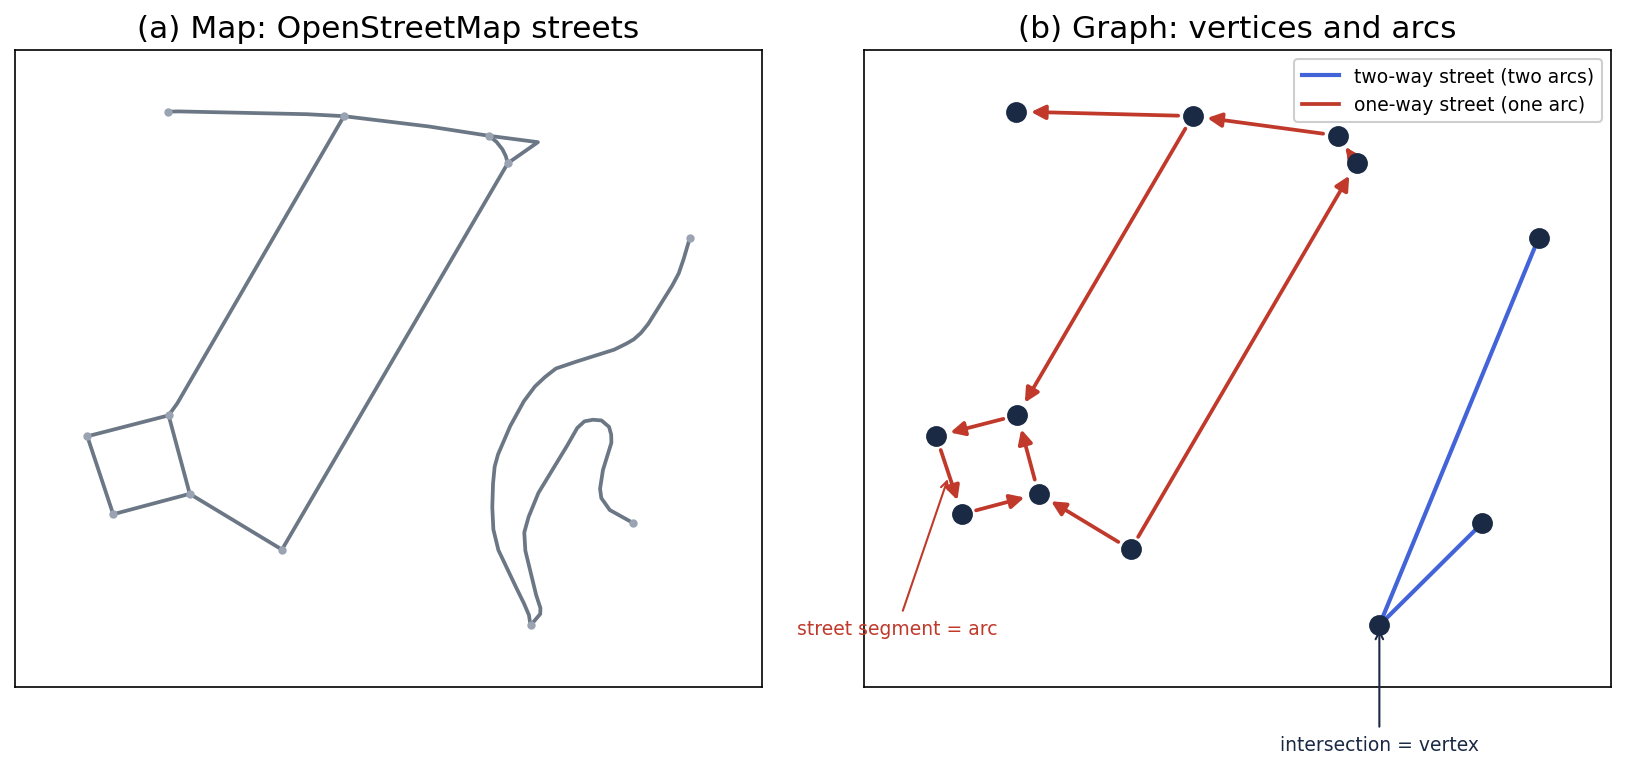
\includegraphics[width=0.8\textwidth]{Figures/fig_construction.png}
\caption{From map to directed graph: intersections become vertices and
street segments become arcs; a one-way street yields a single arc (arrow),
a two-way street two opposite arcs.}
\label{fig:construction}
\end{figure}

The extent of a neighbourhood is a modelling choice. We take the official
polygon (Instituto Pereira Passos / Data.Rio~\cite{ipp_bairros}, retrieved in
September 2026) as the boundary in all three cases. A hand-drawn bounding box
serves only as a search envelope, unioned with the polygon's own bounding box,
and the graph is clipped to the polygon before any analysis, so that no
difference between the neighbourhoods stems from unequal pre-processing.
Streets that cross the boundary are cut there and serve only to identify
gateways (Section~\ref{sec:access-flow}). Section~\ref{sec:res-clip} compares
the outcome with the hand-drawn box alone. Table~\ref{tab:redes} and
Figure~\ref{fig:networks} describe the resulting networks.

\begin{table}[t]
\centering
\caption{Networks after topological simplification (OpenStreetMap), all
three clipped to the neighbourhood's official administrative polygon.}
\label{tab:redes}
\begin{tabular}{lrrr}
\toprule
 & Urca & Copacabana & Botafogo \\
\midrule
Intersections ($V$)                & 70   & 345  & 434 \\
Street segments                    & 104  & 494  & 563 \\
One-way segments (\%)              & 91.3 & 74.9 & 76.2 \\
Strongly connected core ($V$)      & 65   & 331  & 392 \\
Outside the giant core (\% of $V$) & 7.1  & 4.1  & 9.7 \\
\bottomrule
\end{tabular}
\end{table}

\begin{figure}[t]
\centering
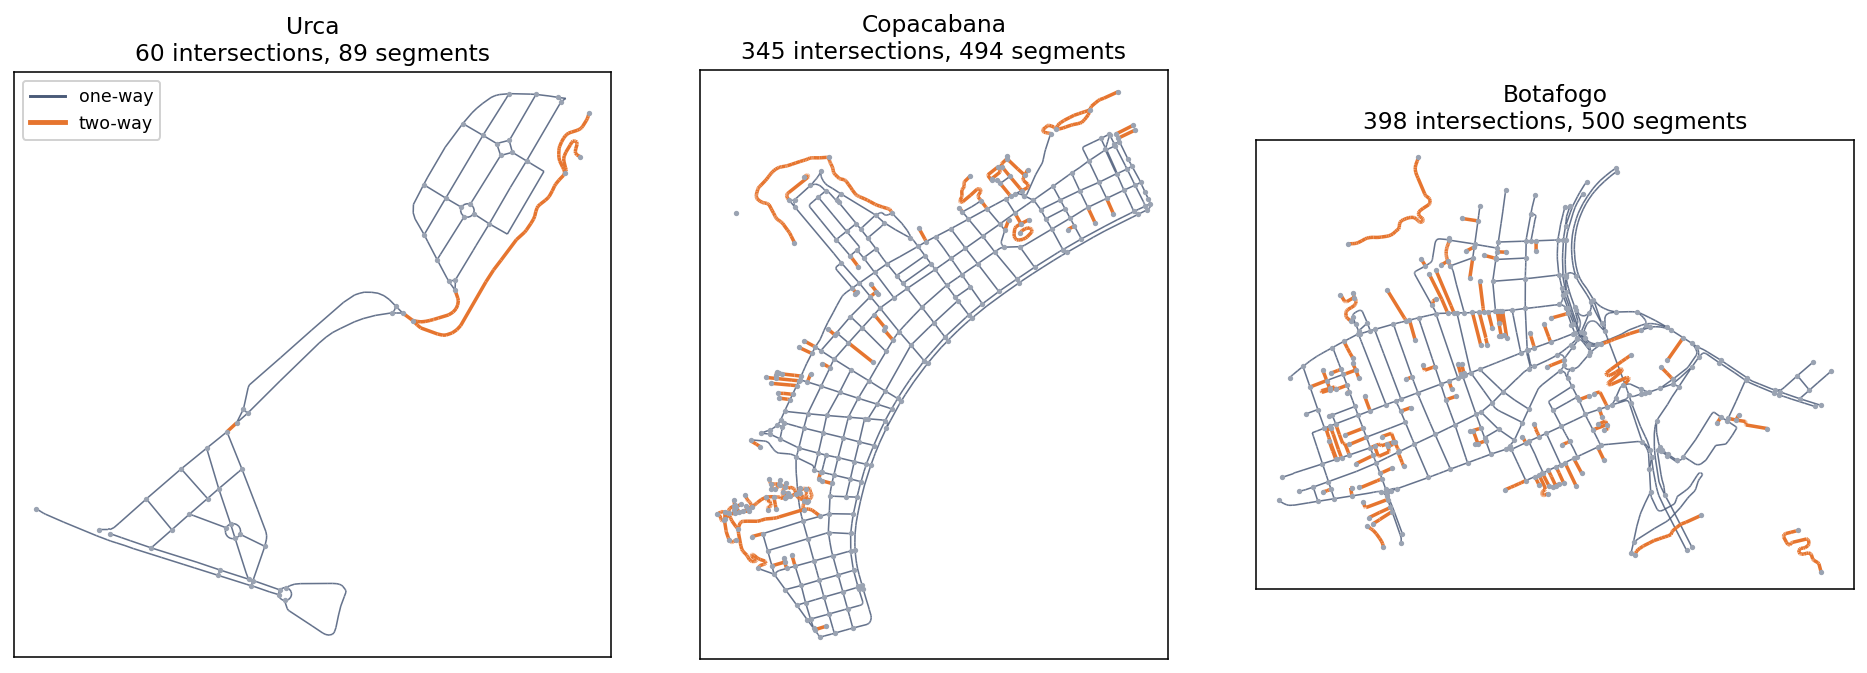
\includegraphics[width=\textwidth]{Figures/fig_networks.png}
\caption{The three neighbourhood networks after topological simplification
and clipping to the official polygon (one-way in dark, two-way in orange).
Urca is a peninsula whose two grids meet at a single corridor; Copacabana
and Botafogo are large open grids.}
\label{fig:networks}
\end{figure}

\subsection{Structural Indicators and Algorithms}
\label{sec:algos}

We compute four structural indicators, each as a proportion
(Table~\ref{tab:estrutural}). Weak bridges are streets whose removal
disconnects the undirected graph, as a percentage of all street segments. The
strongly connected core is the largest strongly connected component (SCC).
Strong bridges are streets whose closure leaves the core no longer strongly
connected, and strong articulation points are intersections whose removal
does~\cite{italiano2012finding}; they are reported as a percentage of the street
pairs and of the intersections of the core. The fourth indicator is the share
of intersections outside the core. Closing a street removes both directions and
any parallel segments between its two intersections; parallel streets are
never weak bridges, and each has unit capacity in the flow computations.

All analyses use a directed, weighted adjacency-list graph. Components are
found by breadth-first search, SCCs by intersecting forward and backward
reachability, and weak bridges and articulation points from their definition.
Strong bridges and articulation points are found by recomputing the SCCs after
each removal, not with the linear-time algorithm of Italiano et al.; this took
0.1\,s, 4.2\,s and 10.2\,s for Urca, Copacabana and Botafogo. Maximum flow and
minimum cut use Edmonds--Karp~\cite{edmonds1972theoretical} with unit capacity
per street in both directions, so that the flow equals the number of
street-disjoint routes. Betweenness follows Brandes~\cite{brandes2001faster},
with Dijkstra's algorithm~\cite{dijkstra1959note} for the travel-time weights;
it is computed on the strongly connected core, splits ties, excludes the
endpoints and is normalised by $(n-1)(n-2)$.

We checked the implementations against \texttt{networkx} on the three networks
(\texttt{test\_vs\_networkx.py}, \texttt{test\_betweenness.py}). Components, SCCs,
weak bridges and articulation points, shortest paths, maximum flow and
betweenness agree. Strong bridges and articulation points, which
\texttt{networkx} lacks, agree with an independent recount of the SCCs after
each removal.

\subsection{Gateway Access Flow}
\label{sec:access-flow}

To measure access to the rest of the city, rather than the separation of two
chosen intersections, we distinguish a neighbourhood's \emph{interior} from its
\emph{gateways}. The street network is also extracted with a 400\,m margin
beyond the official polygon, so that the first intersection beyond the boundary
is present on every street that crosses it. A vertex of the clipped network is
a \emph{gateway} if at least one of its incident streets crosses the boundary;
every other vertex is \emph{interior}. Because a gateway may admit traffic in
only one direction, we restrict both sets to the largest \emph{undirected}
component, not to the strongly connected core: a one-way exit is still a real
way out.

The source region is the $k=\mathrm{round}(f\,n)$ interior intersections
farthest, in number of edges, from the nearest gateway, where $n$ is the size of
that component and $f=0.2$; it is the neighbourhood's core. A super-source feeds
the source region and the gateway set feeds a super-sink, both with infinite
capacity, and Edmonds--Karp is run between them. The resulting value, the
\emph{access flow}, is the number of street-disjoint routes between the core and
the exits to the rest of the city.

\subsection{Controls and Sensitivity Analyses}
\label{sec:controls}

\emph{Node-to-node minimum cut.} As a baseline, we compute the minimum cut
between 300 random pairs of intersections in the largest undirected component
of each network.

\emph{Location of the access cut.} A minimum cut is not unique, and the one that
Edmonds--Karp returns is the closest to the source. We also enumerate every
street whose closure alone separates the source region from all gateways, count
the intersections on each side, and check whether their end intersections
coincide with the five most central ones by betweenness. We repeat this for $f$
from 0.05 to 0.5.

\emph{Size controls.} For the access flow, we draw connected pieces of 70
intersections, Urca's size, inside Copacabana and Botafogo, treat each as a
neighbourhood and compute its access flow; its gateways are its intersections
with a street to an intersection outside it. We draw 500 pieces per
neighbourhood by breadth-first growth and 500 by random growth (Eden model), and
add a hill-climbing search that swaps one intersection at a time to minimise the
flow (8 restarts of 1\,500 iterations). For the betweenness maximum, we draw 300
connected pieces of 65 to 78 intersections per neighbourhood and growth rule,
keep those whose strongly connected core has 60 to 70 vertices (Urca's has 65),
and compare Urca's maximum with theirs. We also compute the product of the
maximum and $\sqrt{n}$, and rewire the edges of each core preserving degrees (50
rewirings per network, undirected and unweighted).

\emph{Extent, source fraction, margin and tunnels.} We repeat the analysis with
the hand-drawn box, unclipped and with the gateways on the box's edge, and vary
$f$ (0.15, 0.20, 0.25) and the margin (200, 400 and 800\,m). A gateway is a
tunnel exit when its exit street runs within 2\,m of a node of a way tagged
\texttt{tunnel=yes} or \texttt{building\_passage}; we recompute the flow without
these gateways. All random procedures use fixed seeds, and the README of the
repository (withheld for review) lists the script for each table and figure.

% =====================================================================
\section{Results}
\label{sec:results}

\subsection{Structural Indicators Do Not Order the Cases}
\label{sec:res-struct}

Table~\ref{tab:estrutural} reports the directed structural indicators as
proportions. They do not order the cases. Botafogo has more strong bridges than
Urca (68.4\% against 61.5\% of core streets), more weak bridges (20.2\% against
10.6\%) and more intersections outside the strong core (9.7\% against 7.1\%);
only on strong articulations does Urca come first (73.8\%, against 63.5\% and
54.1\%). The closest pair changes with the indicator: Urca and Botafogo on
strong bridges and on the outside-core share, Copacabana and Botafogo on weak
bridges and strong articulations. Copacabana, not Urca, stands apart on strong
bridges (45.3\%), and its difference from Botafogo persists when the networks
are built from the hand-drawn box (Section~\ref{sec:res-clip}). In every
neighbourhood, 45\% to 68\% of the core streets are strong bridges; in Urca, 59
of the 96 core streets are, spread over the whole core.

\begin{table}[t]
\centering
\caption{Directed structural indicators (normalised), with all three
networks clipped to the official polygon.}
\label{tab:estrutural}
\begin{tabular}{lrrr}
\toprule
 & Urca & Copacabana & Botafogo \\
\midrule
Weak bridges (\% of segments)       & 10.6 & 15.8 & 20.2 \\
Strong bridges (\% of core streets) & 61.5 & 45.3 & 68.4 \\
Strong articulations (\% of core)   & 73.8 & 54.1 & 63.5 \\
Outside the strong core (\% of $V$) & 7.1  & 4.1  & 9.7 \\
\bottomrule
\end{tabular}
\end{table}

\subsection{The Node-to-Node Minimum Cut Is Small Everywhere}
\label{sec:res-mincut}

Over 300 random pairs of intersections per neighbourhood
(Section~\ref{sec:controls}), the minimum cut is 1 for 70.0\% of the pairs in
Urca, 40.7\% in Copacabana and 52.0\% in Botafogo. The means are 1.49, 1.98 and
1.69, and no pair needs more than 4 streets to be separated. The values are
small in all three and the distributions overlap, so the node-to-node cut does
not separate the cases as the access flow does (Section~\ref{sec:res-access}).

\subsection{The Gateway Access Flow Separates Urca}
\label{sec:res-access}

The access flow (Table~\ref{tab:acesso}) is 1 in Urca, 18 in Copacabana and 15
in Botafogo, through 3, 21 and 31 gateways. The three values are identical for
$f \in [0.15,0.25]$ and for margins from 200 to 800\,m. The structural
indicators and the node-to-node cut do not separate Urca from both open grids
(Sections~\ref{sec:res-struct} and \ref{sec:res-mincut}); the betweenness
maximum does, but it does not survive the size control
(Section~\ref{sec:res-betweenness}), while the access flow does
(Section~\ref{sec:res-cut}). Copacabana's two tunnels, Velho and Novo, account
for four of its 21 gateways (those whose exit street runs through a way tagged
\texttt{tunnel}); without them its access flow is 15. The same tunnels give
Botafogo four gateways, and its flow stays at 15.

\begin{table}[t]
\centering
\caption{Gateway access flow: street-disjoint routes from each
neighbourhood's core to its administrative gateways ($f=0.2$; the values
are stable over the ranges of $f$ and margin in Section~\ref{sec:controls}).}
\label{tab:acesso}
\begin{tabular}{lrrr}
\toprule
 & Urca & Copacabana & Botafogo \\
\midrule
Gateways identified              & 3    & 21             & 31 \\
Access flow (routes)             & 1    & 18             & 15 \\
\bottomrule
\end{tabular}
\end{table}

\subsection{Location of the Cut and Size Controls}
\label{sec:res-cut}

Figure~\ref{fig:cut} shows the cuts (Section~\ref{sec:controls}). In Urca there
are three single-street cuts, in series, all on the corridor that joins the two
residential grids: a 165\,m street at its north-eastern end (the cut
Edmonds--Karp returns), a 32\,m street adjacent to it, and a 33\,m street at its
south-western junction. None lies inside a residential grid, and they leave 23,
27 and 33 of the 70 intersections (33\% to 47\%) on the source side. Three
single-street cuts, all ending on the same five intersections, are found for
every $f$ from 0.05 to 0.25; for larger $f$ the source region reaches the
corridor and the cuts disappear one by one (none remains at $f=0.5$).
Copacabana and Botafogo have no single-street cut: their minimum cuts have 18
and 15 streets spread across the neighbourhood.

\begin{figure}[t]
\centering
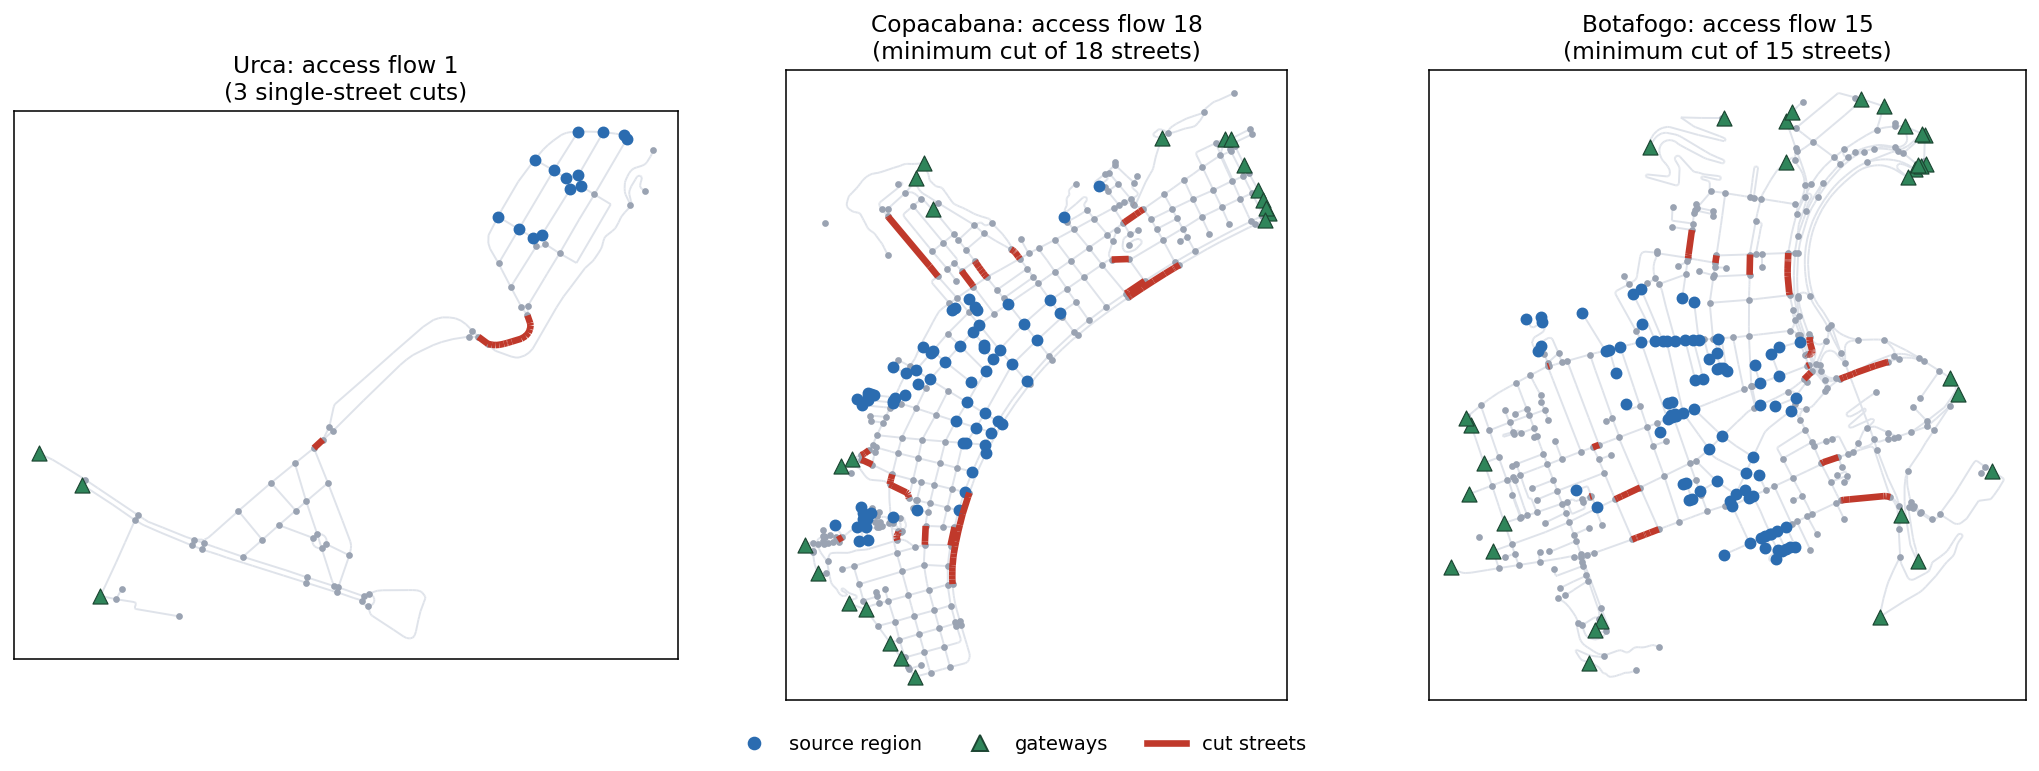
\includegraphics[width=\textwidth]{Figures/fig_cut.png}
\caption{Where the access cut lies ($f=0.2$). Blue: source region; green:
gateways; red: cut streets. In Urca the three single-street cuts all lie on
the corridor between the two grids; in Copacabana and Botafogo the minimum
cut (18 and 15 streets) is spread across the neighbourhood.}
\label{fig:cut}
\end{figure}

None of the 2\,000 pieces of 70 intersections drawn inside Copacabana and
Botafogo reached a flow of 1 (Figure~\ref{fig:controles}a). The median flow was 8 to 13, every piece had at
least 9 gateways (Urca has 3), and pieces with a flow of 3 or less were 17\%
and 11\% of the Copacabana pieces and 0\% and 0.2\% of the Botafogo pieces. The
hill-climbing search found no piece below 3 (with 53 and 45 gateways). The
pieces are arbitrary cuts, not real neighbourhoods, and the search gives a
heuristic bound, not a proof.

\begin{figure}[t]
\centering
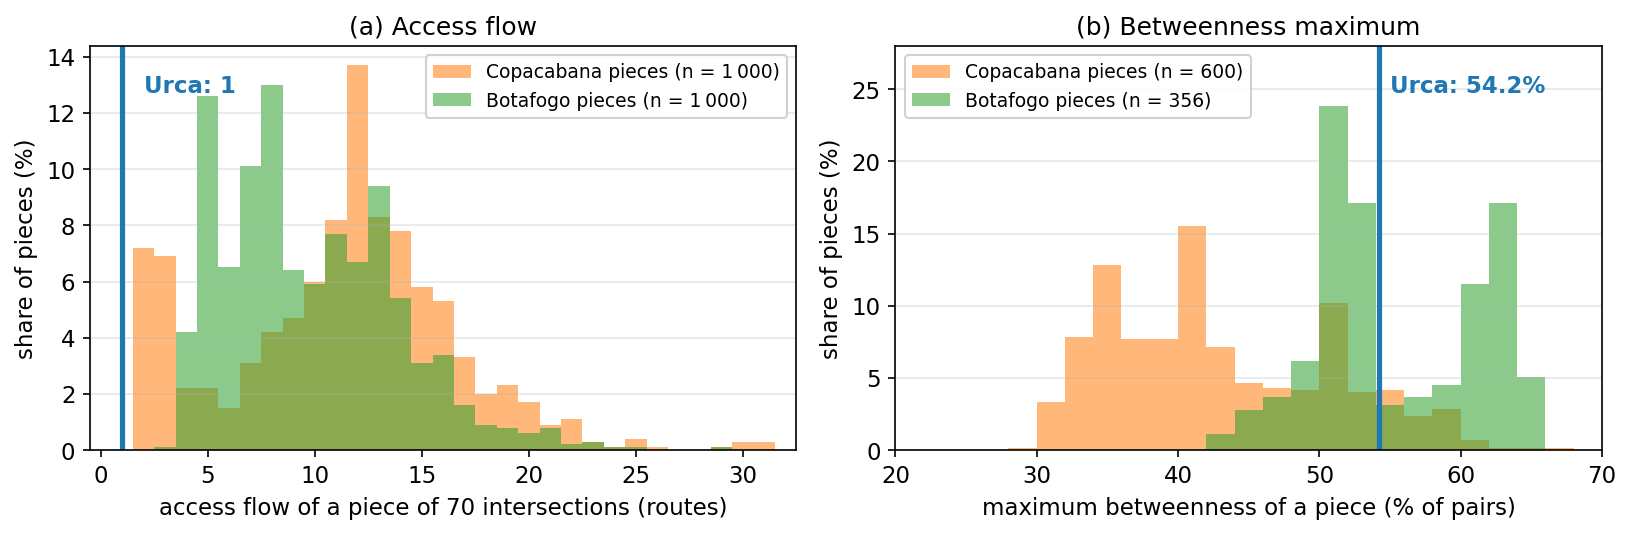
\includegraphics[width=\textwidth]{Figures/fig_controles.png}
\caption{Size controls. (a) Access flow of connected pieces of 70
intersections drawn inside Copacabana and Botafogo (500 by breadth-first
growth and 500 by random growth each); Urca's flow is 1. (b) Betweenness
maximum of the size-matched pieces (Section~\ref{sec:controls}); Urca's is
54.2\%.}
\label{fig:controles}
\end{figure}

\subsection{Betweenness Locates the Corridor but Does Not Separate the Cases}
\label{sec:res-betweenness}

Directed betweenness (Figure~\ref{fig:betweenness}) peaks in Urca on five
intersections along the corridor and at its junctions with the two grids, which
lie on 45.8\% to 54.2\% of all ordered pairs; they are exactly the endpoints of
the three single-street cuts. In Copacabana and Botafogo the maxima are 27.8\%
and 22.4\%, along the main axis of Copacabana and along two parallel streets in
Botafogo.

The magnitude does not separate the cases once size is taken into account. If
the maximum scaled as $n^{-1/2}$, its product with $\sqrt{n}$ would be
constant; it is nearly so (4.4 in Urca, 5.1 in Copacabana, 4.4 in Botafogo). In
the size-matched null (Section~\ref{sec:controls}, Figure~\ref{fig:controles}b), Urca's 54.2\% is exceeded by
44\% to 52\% of the Botafogo pieces and by 2\% to 18\% of the Copacabana pieces,
depending on the growth rule ($z$-scores from $-0.3$ to 1.9; the random-growth
Botafogo null has 56 pieces). Rewiring the edges while preserving degrees gives
$z$-scores of 22 to 39 for all three neighbourhoods.

\begin{figure}[!htb]
\centering
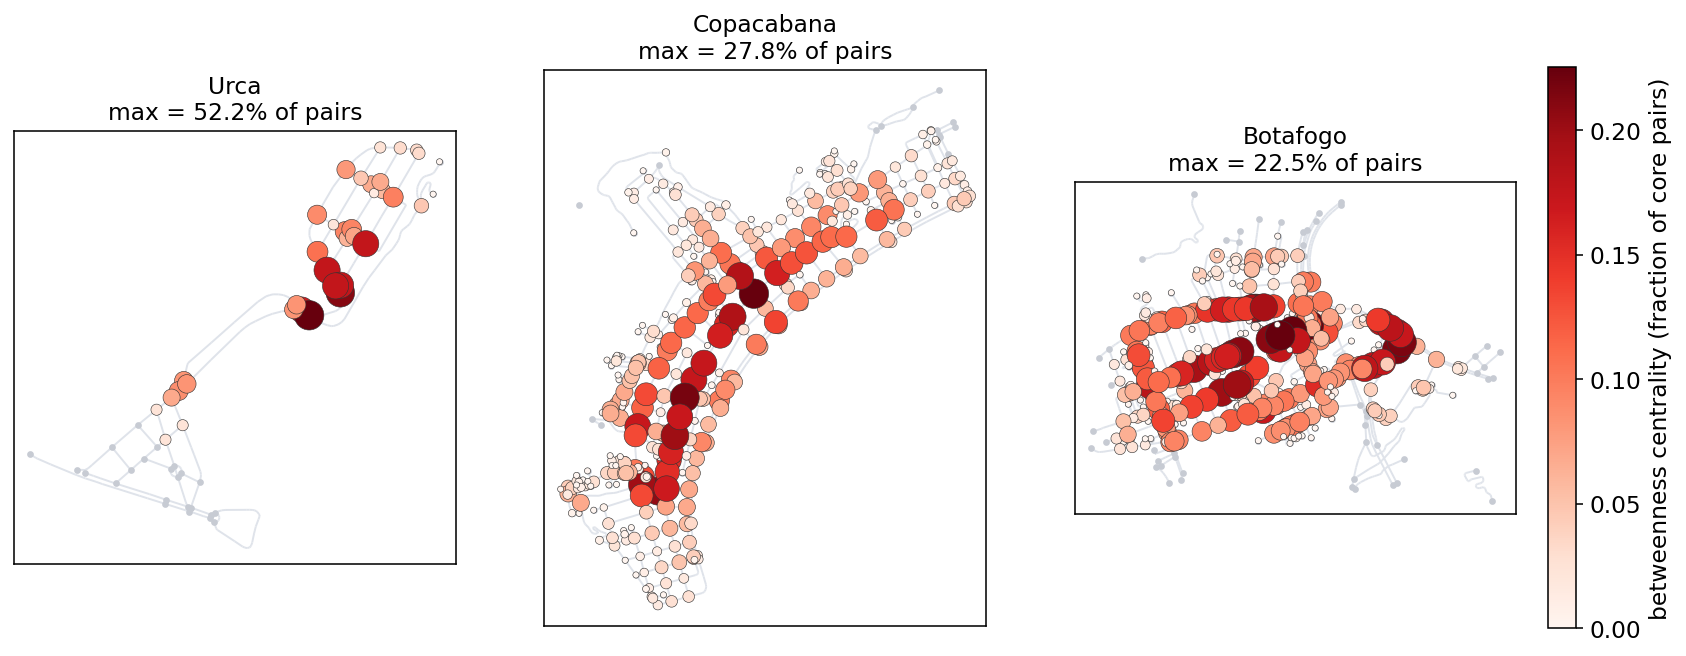
\includegraphics[width=\textwidth]{Figures/fig_betweenness.png}
\caption{Directed betweenness centrality (shortest-time paths, strong core),
on a common colour scale. The maxima are not comparable across core sizes (see
text).}
\label{fig:betweenness}
\end{figure}

\subsection{Sensitivity to the Type of Clip}
\label{sec:res-clip}

Table~\ref{tab:recorte} repeats the central measures with the hand-drawn box,
unclipped and with the gateway boundary defined by the box itself, and with the
official polygon. The clip barely affects Botafogo (strong bridges from 70.4\%
to 68.4\%; access flow from 16 to 15). In Copacabana the box included 158 of
its 496 intersections that lie in Botafogo's official territory; clipping lowers
strong bridges from 53.1\% to 45.3\% and gateways from 45 to 21. In Urca the box
truncated the peninsula; clipping takes the strong core from 37 to 65
intersections and the share outside it from 38.3\% to 7.1\%. The strong-bridge
gap between Copacabana and Botafogo exists under both clips (53.1\% against
70.4\% with the box; 45.3\% against 68.4\% with the polygon), and the access flow
separates Urca under both (1, against 13 to 18 in Copacabana and 15 to 16 in
Botafogo). The share of Urca intersections outside the strong core and the
number of gateways depend on the clip.

\begin{table}[t]
\centering
\caption{Sensitivity to the type of clip. Box: hand-drawn box, unclipped,
with gateways on the box's edge. Polygon: official polygon (the paper's
version). $V$: intersections; Out: \% of $V$ outside the strong core;
Bridges: \% of strong bridges; Flow: access flow ($f=0.2$).}
\label{tab:recorte}
\footnotesize
\setlength{\tabcolsep}{4pt}
\begin{tabular}{llrrrrr}
\toprule
Neighbourhood & Clip & $V$ & Out & Bridges & Gateways & Flow \\
\midrule
Urca       & box     & 60  & 38.3 & 67.3 & 4  & 1  \\
           & polygon & 70  & 7.1  & 61.5 & 3  & 1  \\
\midrule
Copacabana & box     & 496 & 19.6 & 53.1 & 45 & 13 \\
           & polygon & 345 & 4.1  & 45.3 & 21 & 18 \\
\midrule
Botafogo   & box     & 398 & 14.3 & 70.4 & 28 & 16 \\
           & polygon & 434 & 9.7  & 68.4 & 31 & 15 \\
\bottomrule
\end{tabular}
\end{table}

% =====================================================================
\section{Discussion}
\label{sec:discussion}

The structural indicators do not order the three neighbourhoods, and Urca stands
out, once size is controlled, only in the access flow. This fits how they are
built. Strong bridges and
articulation points are computed on the strongly connected core alone, and in
these one-way networks 45\% to 68\% of the core streets are strong bridges, so
they describe redundancy inside the core, not its connection to the rest of the
city. The node-to-node minimum cut answers another question, how many streets
separate two chosen points. The access flow takes the core as source and the
boundary crossings as sink, and so measures that connection.

In Urca, the flow of 1 is a corridor: three single-street cuts in series, a set
that, as Sugiura and Kurauchi note for isolation
vulnerability~\cite{sugiura2023isolation}, need not be unique. Pieces of the
open grids with Urca's size do not reach a flow of 1, which places the
difference in the boundary: few exits, all at one end. The betweenness maximum,
by contrast, tracks core size in these data, so it locates the corridor but
cannot compare the neighbourhoods. Copacabana's tunnels do not create a
comparable bottleneck: removing its four tunnel gateways lowers the flow only
from 18 to 15.

The study has three cases and is illustrative, not statistically general; the
single-route pattern appears in Urca and in neither of the two open grids
studied. The access flow treats every street as two-way with unit capacity, so
it ignores one-way direction, width and lanes, and a directed version was not
computed. The extent is a modelling choice, as the hand-drawn box showed
(Section~\ref{sec:res-clip}), and an administrative boundary is not necessarily
a mobility unit. Travel times, used only by betweenness, are mostly default
speeds, and the connectivity indicators depend on the quality of the
\texttt{oneway} tags. The size-matched pieces are arbitrary cuts, not
neighbourhoods.

\FloatBarrier

% =====================================================================
\section{Conclusion}
\label{sec:conclusion}

Among the measures tested, only the gateway access flow distinguishes Urca
from the two open grids: one street-disjoint route against eighteen in
Copacabana and fifteen in Botafogo, an ordering stable under variations of the
clip, the margin and the source region. The directed structural indicators
that motivate the paper's framing, strong bridges and strong articulation
points, do not order the three neighbourhoods, and the node-to-node minimum
cut is small in all three; the measure that does separate the cases is
computed on the undirected network. The distinction tracks geography rather
than size: Urca's cut lies on the corridor between its two grids, pieces of
the open grids with Urca's size do not reproduce a flow of 1, and removing
Copacabana's four tunnel gateways still leaves a flow of fifteen. The
single-route pattern therefore appears in the peninsula and in neither open
grid studied. These observations rest on three contrasting cases and are
illustrative, not statistically general; extending the comparison to more
neighbourhoods, computing the flow on the directed network, and correlating it
with a geometric shape index are left for future work. Practically, a route
count of this kind could help a mobility or civil-defence authority flag a
neighbourhood with only one way out.

\subsubsection*{Reproducibility.} All source code and data are openly
available (repository withheld for double-blind review).

% =====================================================================
\bibliographystyle{splncs04}
\bibliography{references}
% Bibliografia em references.bib. NOVAS entradas a acrescentar (ver aviso
% no final da resposta): hillier1984social, ipp_bairros.

\end{document}
